
Consider the canonical signal-plus-noise model where the observation $x$ is a high-dimensional vector in $\R^p$,
\begin{equation} \label{eq:model}
    x = \mu + \epsilon.
\end{equation}
The signal, $\mu = (\mu(j))_{j=1}^p$, is a vector with $s$ non-zero components supported on the set $S=\{j:\mu(j)\neq 0\}$; the second term $\epsilon$ is a random error vector. 
The goal of high-dimensional statistics is usually two-fold: 
\begin{enumerate}
    \item To detect the presence of non-zero components in $\mu$. That is, to test the global hypothesis $\mu = 0$, which we call the \emph{detection} problem, and
    \item To estimate the support set $S$, which we call the \emph{support recovery} problem.
\end{enumerate}
An archetypal application where the two problems arise is in cyber security \citep{kallitsis2016amon}.
Internet service providers routinely collect statistics of server to determine if there are abnormal surges or blackouts.
% The ISPs collect, for example, incoming traffic volumes to each server to determine if there are abnormal surges or blackouts.
While this monitoring is performed over a large number of servers, only very few servers are believed to be experiencing problems at any time.
The signal detection problem is then equivalent to determining if there are any anomalies among all servers; the support recovery problem is equivalent to identifying the servers with anomalies.

The same two questions are pursued in, for example, large-scale microarray experiments \citep{dudoit2003multiple}, brain imaging and fMRI analysis \citep{nichols2003controlling}, and numerous other applications.

A common theme in such applications is that the error terms are correlated, and that the signal vectors are believed to be sparse: the number of non-zero components in $\mu$ is small compared to the number of test performed.
Under such dependence and  sparsity assumptions, it is natural to ask if and when one can reliably {(1)} detect the signals, and {(2)} recover the support set $S$.
% Further, one would like to characterize the statistical procedures that achieve efficient detection and support recovery, whenever such goals become possible to achieve.
In this paper, we focus on the support recovery problem, and seek minimal conditions under which the support set can be consistently estimated.

\subsection{Set-up} \label{subsec:set-up}

We now describe the models and assumptions that we are going to work with for the rest of the paper.

\subsubsection{Assumptions on the error distributions}

We assume that the errors come from a triangular array
\begin{equation}
\label{eq:error-array}
{\cal E} = \left\{ (\epsilon_p(j))_{j=1}^p,\ p=1,2,\dots\right\},
\end{equation}
such that the $\epsilon_p(j)$'s have common distribution $F$.

We shall consider light-tailed error distributions with {\em rapidly varying} tails (see e.g.,\ Definition \ref{def:rapid-variation} below). 
To be concrete and better convey the main ideas, we will focus on the class of asymptotically generalized Gaussian laws (see Definition \ref{def:AGG}), which is still a fairly general class of models commonly used in the literature on high-dimensional testing \citep{cai2007estimation, arias2017distribution}.
Extensions to other models are deferred to Appendix \ref{sec:other-boundaries}.

\begin{definition} \label{def:AGG}
A distribution $F$ is called asymptotic generalized Gaussian with parameter $\nu$ (denoted $\text{AGG}(\nu)$) if
\begin{enumerate}
    \item $F(x)\in(0,1)$ for all $x\in\R$, and \smallskip
    \item $\log{\overline{F}(x)} \sim -\frac{1}{\nu}x^\nu$ and $\log{F(-x)} \sim -\frac{1}{\nu}(-x)^\nu,$ \label{eq:AGG}
\end{enumerate}
where $\overline{F}(x) = 1 - F(x)$ is the survival function, and $a(x)\sim b(x)$ is taken to mean $\lim_{x\to\infty} a(x)/b(x) = 1$.
\end{definition}

The AGG models include, for example, the Gaussian distribution ($\nu = 2$), and the Laplace distribution ($\nu = 1$) as special cases. 
Since the requirement is only placed on the tail behavior, this class encompasses a large variety of light-tailed models.

On the other hand, the AGG model are themselves special cases of a more general class of tail models as we will see in Example \ref{exmp:AGG}.
For simplicity of exposition, however, we shall focus on the $\text{AGG}(\nu)$ distributions, where the quantiles have explicit expressions.
\begin{proposition} \label{prop:quantile}
The the $(1/p)$-th upper quantile of $\text{AGG}(\nu)$ is
\begin{equation} \label{eq:AGG-quantiles}
    u_{p} := F^\leftarrow(1-1/p) \sim \left(\nu\log{p}\right)^{1/\nu},
\end{equation}
where $F^\leftarrow(q) = \inf_x\{x:F(x)\ge q\},\ q\in (0,1)$.
\end{proposition}
The proof of Proposition \ref{prop:quantile} can be found in Appendix \ref{sec:AGG}.
% We remark here that the family of density is log-concave for $\nu \ge 1$, therefore the oracle procedure is the thresholding procedure (See Section \ref{subsec:oracle}).

Note that the errors are only assumed to have common marginal distributions, and may have potentially arbitrary dependence.
We will study the role of dependence in support recovery problems in Section \ref{sec:URS}. 

\subsubsection{Assumptions on the signals}
We assume in model \eqref{eq:model} that $\mu = \left(\mu(j)\right)_{j=1}^p$ is a sparse signal vector with non-zero entries only at the support of the signal $S_p\subseteq \{1,\ldots,p\}$. 
We denote the size of the support set as $s = |S_p|$, and assume that the non-zero entries of $\mu$ are positive and take values in the interval $\left[\underline{\Delta},\overline{\Delta},\right]\subset(0,\infty)$.

Following \citep{ingster1998minimax, donoho2004higher, cai2007estimation, haupt2011distilled, arias2017distribution}, we parametrize the signal sparsity as
\begin{equation} \label{eq:sparsity-parametrized}
    s = s(p) = \lfloor p^{1-\beta} \rfloor, % \quad \text{with } 0 < \beta \le 1 \; \text{(fixed)},
\end{equation}
with $0 < \beta \le 1$ fixed. We also parametrize the signal sizes $\underline{\Delta}$ and $\overline{\Delta}$ as
\begin{equation} \label{eq:signal-size-parametrized}
    \underline{\Delta} = \underline{\Delta}(p) = (\nu \underline{r} \log{p})^{1/\nu} \quad \text{and} \quad
    \overline{\Delta} = \overline{\Delta}(p)  = (\nu \overline{r} \log{p})^{1/\nu},
\end{equation}
with parameters $0 < \underline{r} \le \overline{r}$.

\subsection{Thresholding procedures} \label{subsec:thresholding-procedures}

We review four procedures that will be analyzed in this paper.
All of them fall under the class of thresholding procedures, which we define as follows.
\begin{definition}[Thresholding procedures]
A thresholding procedure for estimating the support 
$S_p:=\{j\, :\, \mu(j)\neq0\}$ is one that takes on the form
\begin{equation} \label{eq:thresholding-procedure}
    \widehat{S}_p = \left\{j\, :\, x(j) > t_p(x)\right\}.
\end{equation}
We note here that the threshold $t_p(x)$ may depend on the data $x$.
\end{definition}
A well-known (deterministic) thresholding procedure is Bonferroni's procedure.
\begin{definition}[Bonferroni's procedure]
Suppose the errors $\epsilon(j)$'s have a common marginal distribution $F$, Bonferroni's procedure with family-wise error rate (FWER) at most $\alpha$ is the thresholding procedure that uses the threshold
\begin{equation} \label{eq:Bonferroni-procedure}
    t_p = F^{\leftarrow}(1 - \alpha/p).
\end{equation}
%where  $F^{\leftarrow}(u)=\inf{\left\{x:F(x)\ge u\right\}}$ is the generalized inverse function.
\end{definition}
% It is easy to see that the family-wise error rate (FWER) is controlled at level $\alpha$ by applying the union bound, regardless of the error-dependence structure (see e.g.\ Relation \eqref{eq:Bonferroni-FWER-control}, below).
A closely related procedure is Sid\'ak's procedure \citep{vsidak1967rectangular}
which is a more aggressive (and also deterministic) thresholding procedure that uses the 
threshold
\begin{equation} \label{eq:Sidak-procedure}
    t_p = F^{\leftarrow}((1 - \alpha)^{1/p}).
\end{equation}
% can be shown to control FWER in the case independent errors.

Another procedure, which is strictly more powerful than Bonferroni's, is Holm's procedure \citep{holm1979simple}.
On observing the data $x$, its coordinates can be ordered from largest to smallest
$x(j_1) \ge x(j_2)  \ge \ldots \ge x(j_p)$,
where $(j_1, \ldots, j_p)$ is a permutation of $\{1, \ldots, p\}$. 
\begin{definition}[Holm's procedure]
Let $k$ be the largest index such that
$$
\overline{F}(x(j_i)) \le \alpha / (p-i+1),\quad \text{for all}\;i\le k.
$$
Holm's procedure with FWER controlled at $\alpha$ is the thresholding procedure that uses
\begin{equation} \label{eq:Holm-procedure}
    t_p(x) = x(j_{k}),
\end{equation}
\end{definition}
In contrast to the Bonferroni procedure, Holm's procedure is data-dependent.
% It can be shown that Holm's procedure also controls FWER at $\alpha$ level, regardless of dependence in the data.
A closely related, more aggressive (data-dependent) thresholding procedure is Hochberg's procedure \citep{hochberg1988sharper},
%\begin{definition}[Hochberg's procedure]
%Hochberg's procedure 
which replaces the index $k$ in Holm's with the largest index $i$ such that
$$
\overline{F}(x(j_i)) \le \alpha / (p-i+1).
$$
%where  $\overline{F}(x)=1-F(x)$ is the survival function.
%\end{definition}

We will analyze the performance of these thresholding procedures in Section \ref{sec:sufficient}.
The (sub)optimality of general data-dependent thresholding procedures will be established in Section \ref{subsec:optimality}.
We now return to the discussion of support recovery.

\subsection{The Hamming-loss approach and its deficiencies}
Recall our goal is to establish minimal conditions under which the support set can be consistently estimated, i.e.,
\begin{equation} \label{eq:goal}
    \P[\widehat{S}_p = S_p] \longrightarrow 1 \quad \text{as } \; p\to\infty, 
\end{equation}
where $\widehat{S}_p$ is an estimate of the true set of signal support $S_p$.
Previously, the probability of exact support recovery has been studied via the Hamming loss, defined as the number of mismatches between the estimated and true support set,
\begin{equation} \label{eq:Hamming-loss}
    H(\widehat S, S)
    = \left|\widehat S \setminus S\right| + \left|S \setminus \widehat S\right|
    = \sum\limits_{j=1}^p\left|\mathbbm{1}_{\widehat{S}}(j)- \mathbbm{1}_{S}(j)\right|.
\end{equation}
As pointed out in, e.g. \citet{butucea2018variable}, there is a natural lower bound for the probability of support recovery by the expected Hamming loss,
\begin{equation} \label{eq:Hamming-loss-lower-bound}
    \mathbb{P}[\widehat S = S] 
    \ge 1 - \mathbb{E}[H(\widehat S, S)]
    = 1 - \sum\limits_{j=1}^p\E\left|\mathbbm{1}_{\widehat{S}}(j)- \mathbbm{1}_{S}(j)\right|.
\end{equation}
However, vanishing Hamming loss is only sufficient, not necessary for support recovery \eqref{eq:goal}.
A key observation in Relation \eqref{eq:Hamming-loss-lower-bound} is that the expected Hamming loss decouples into $p$ terms, and dependence of the estimates $\mathbbm{1}_{\widehat{S}}(j)$ among the $p$ locations no longer plays a role in the sum.
Therefore, studying support recovery problems via the expected Hamming loss is not very informative especially under severe dependence, as the bound \eqref{eq:Hamming-loss-lower-bound} may become \emph{very} loose.

Despite this deficiency, some intriguing results have been derived for the independent or near-independent case.
For example, \citet{genovese2012comparison} and \citet{ji2012ups} studied the problem of support recovery in linear models under the Hamming loss.
Under the parametrization in \eqref{eq:sparsity-parametrized} and \eqref{eq:signal-size-parametrized}, a minimax-type phase transition result was established. In \citep{ji2012ups}, it was shown that the  Hamming loss diverges to $+\infty$ when signal sizes $r$ fall below the threshold
\begin{equation} \label{eq:strong-classification-boundary-Gaussian}
    g(\beta) = (1 + (1 - \beta)^{1/2})^2,
\end{equation}
for any method of support estimation.
Conversely, under orthogonal, or near-orthogonal random designs, if $r>g(\beta)$, their proposed method achieves vanishing Hamming loss.

Very recently, \citet{butucea2018variable} studied both asymptotics and non-asymptotics of the support recovery problem in the additive noise model \eqref{eq:model} with Gaussian errors under the Hamming loss.
It was again shown that the boundary \eqref{eq:strong-classification-boundary-Gaussian} exists in a minimax sense.
That is, when errors are \emph{independent}, the Hamming loss cannot be made to vanish if signal sizes fall below the boundary \eqref{eq:strong-classification-boundary-Gaussian}. 
Conversely, if $r>g(\beta)$, the Hamming loss can be made to vanish with a particular thresholding procedure.

% See also, Example \ref{exmp:counter-example} and Figure \ref{fig:phase-simulated-very-dependent} (bottom-right panel).

So far in the literature, the role of dependence, and that of the distributional assumptions in the exact support recovery problem remain largely unexplored.  
This is arguably a consequence of the inherent limitation of the Hamming-loss approach. 
The minimax formulation, although elegant, focuses on the independent cases and obviates a fuller exploration of the phenomenon under various dependence conditions.
For practitioners, a minimax statement in the Gaussian case seems to offer little guidance.
Indeed, in applications, independence is an exception rather than the rule; Gaussianity of the errors may also be unnecessarily restrictive.


These considerations motivate us to study the support recovery problem \eqref{eq:goal} directly, under general distributional assumptions and dependence.
In particular, it would be of interest to see if the phase transition continues to hold when we shift our focus from Hamming loss to support recovery \eqref{eq:goal}.
It would interesting to know how dependence may aid in the problem of support recovery, and when boundaries such as $g$ in \eqref{eq:strong-classification-boundary-Gaussian} remain tight under dependent, and possibly non-Gaussian errors.
We provide answers to these questions in this paper. 
Our contributions are summarized in Subsections \ref{subsec:role-of-dependence}, \ref{subsec:role-of-URS}, and \ref{subsec:role-of-thresholding} below.

% In view of the popularity of the FDR-controlling procedures, it is natural to ask if one should still care about the much more stringent exact support recovery at all. 
% We believe the answer to this question is \emph{yes}, since FDR control for support recovery is insufficient in at least three broad areas of applications that we encounter.

% Firstly, FDR-controlling studies are mostly used as first stage screenings, and often require a second-stage confirmatory study. In practice, we often do not have the luxury to perform a follow-up study to confirm the findings filtered by the FDR-controlling procedures. Time-sensitive decisions have to be made there and then, regarding the validity of these support recovery results. 
% Secondly, some applications call for extremely low tolerance of FDP and NDPs, because costs associated with a false positive is extremely high. 
% As an example, the task of Internet traffic monitoring requires careful considerations on both fronts:
% monitoring is performed not only at large number of locations, but also repeatedly over time, even investigating results from a FDR-controlling procedure is prohibitive;
% also, incorrectly filter IP addresses could result in legitimate, and possibly vital traffic being disrupted.
% Lastly, and perhaps most surprisingly, applying FDR control procedures in a repeated testing or monitoring setting fails to control for FDR! We refer readers to the appendix for a details of the last claim.

% Therefore, we believe it would be of interest to understand the arguably overlooked problem of FWER control in high dimensions, and in turn, when \emph{exact} recovery signal supports is possible (i.e., $\mathbb P[\widehat{S} = S] \to 1$), and not just with vanishing fraction of errors (i.e., $\text{FDP} + \text{NDP} \to 0$). 

\subsection{Role of dependence and point-wise phase transitions}
\label{subsec:role-of-dependence}
Consider the function
\begin{equation} \label{eq:strong-classification-boundary}
    g(\beta) = (1 + (1 - \beta)^{1/\nu})^\nu,
\end{equation}
which we refer to as the {\em strong classification boundary}.
In Theorem \ref{thm:sufficient} we show that, under the general distributional assumptions in Section \ref{subsec:set-up}, if the signal size is above the boundary (i.e., $\underline{r}> g(\beta)$), procedures described in Section \ref{subsec:thresholding-procedures} with appropriately calibrated levels achieve perfect support recovery, that is,
\begin{equation} \label{eq:exact-recovery}
    \mathbb{P}\left[\widehat{S}_p=S_p\right]\longrightarrow 1,\quad \mbox{ as }p\to \infty.
\end{equation}

Conversely, we show in Theorem \ref{thm:necessary}, that for a surprisingly large class of dependence structures characterized by the concept of \emph{uniform relative stability} (URS, see Definition \ref{def:URS}), when the signal size is below the boundary  (i.e., $r<g(\beta)$), no thresholding procedure can achieve the asymptotically perfect support recovery \eqref{eq:exact-recovery}. In fact,
\begin{equation} \label{eq:exact-recovery-failure}
    \mathbb{P}\left[\widehat{S}_p=S_p\right]\longrightarrow 0,\quad \mbox{ as }p\to \infty,
\end{equation}
for all $\widehat{S}_p$ in the form of \eqref{eq:thresholding-procedure}.

Complementing results in \citet{butucea2018variable}, these two results show that the thresholding procedures obey a phase transition phenomenon in a strong, \emph{point-wise} sense over the class of URS dependence structures, and over the class of AGG$(\nu),\ \nu>0$ error distributions. 

The strong classification boundary $g$ characterizes a phase-transition phenomenon similar to that of the signal detection, and approximate support recovery. 
A preview of this result is presented in Figure \ref{fig:phase}, which shows the boundaries for signal detection, approximate support recovery, and exact support recovery, in the special case of Gaussian and Laplace errors, respectively. 

\subsection{Uniform relative stability and concentration of maxima}
\label{subsec:role-of-URS}
The key probabilistic concept behind our characterization of the dependence structure under which \eqref{eq:exact-recovery-failure} takes place is a certain {\em concentration of maxima} phenomenon, known as {\em relative stability} (see Section \ref{sec:URS}).
We introduce and study an extension of this concept referred to as uniform relative stability (URS). 
Broadly speaking, the strong classification boundary phenomenon holds for dependent light-tailed errors, provided that they are uniformly relatively stable. 

In the case of dependent Gaussian errors, we establish in Theorem \ref{thm:Gaussian-weak-dependence} a complete characterization of URS in terms of a simple condition on the covariance structure, using the Sudakov-Fernique bounds and a curious application of Ramsey theory.
These results may be of independent interest, since they characterize Gaussian triangular arrays whose maxima concentrate at the same rate as in the case of independence.

\begin{figure}
      \centering
      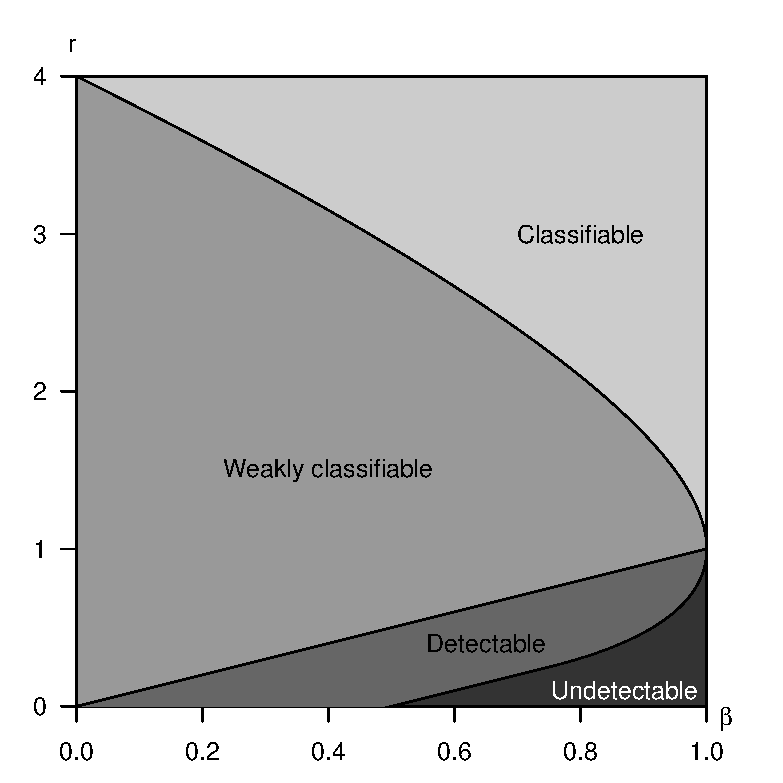
\includegraphics[width=0.45\textwidth]{./figures/phase_diagram_Gaussian_no_dashed_area.eps}
      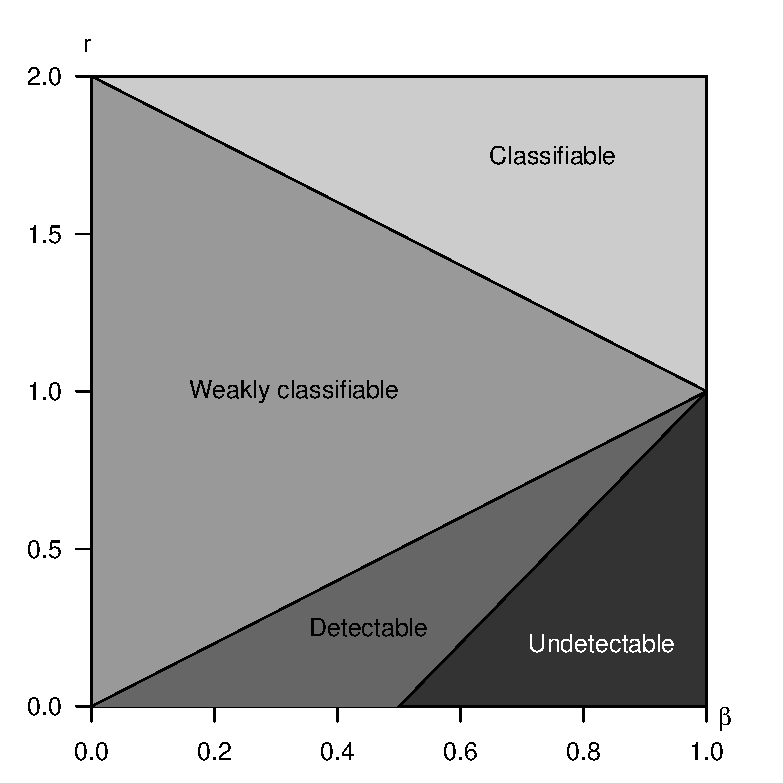
\includegraphics[width=0.45\textwidth]{./figures/phase_diagram_double_exponential.eps}
      \caption{The phase diagrams of the detection, weak classification, and strong classification boundaries against sparse alternatives under Gaussian (left) and Laplace distributed (right) errors. The parameters $\beta$ and $r$ parametrize the signal sparsity and signal size, respectively.
      %The signal detection problem can be answered perfectly (asymptotically) inside the \emph{Detectable} region;
      %False discovery proportion and non-discovery proportion can be made to vanish in the \emph{Weakly classifiable} region. 
      We study in this paper the strong classification boundary, above which the support recovery can be achieved \emph{exactly} in the \emph{Classifiable} region. In a large class of dependence structures characterized by URS, when signal sizes fall below the strong classification boundary, no thresholding procedure succeeds in the exact support recovery problem.
      For the detection and weak classification boundaries, see, e.g., \citep{haupt2011distilled, arias2017distribution, ingster1998minimax, donoho2004higher}, and Sec \ref{sec:sufficient}.}
      \label{fig:phase}
\end{figure}

\subsection{Role of thresholding procedures and minimax optimality}
\label{subsec:role-of-thresholding}
In Section \ref{subsec:optimality}, we show that the thresholding procedures are Bayes optimal when the errors independent and identically distributed with log-concave density. 
In this case, no estimator can achieve perfect support recovery when the signal is below the strong classification boundary \eqref{eq:strong-classification-boundary}.  
Consequently, in the case of $(\nu\ge 1)$, the strong 
classification boundary is shown to hold in the minimax 
sense for \emph{all} procedures. This is formalized in Theorem \ref{thm:necessary-strengthened}. 

We further clarify the roles played by thresholding procedures in support recovery problems.
% In the problem of global testing, \citet*{arias2018detection} observed that when errors follow a power-law distribution, the top observations do not contribute much to the power in testing for the presence of sparse mixtures.
We show that thresholding procedures (including data-dependent ones) are not optimal in general in the support recovery problem when the errors have super-exponential tails. See also, \citet*{arias2018detection}.
In this case, the presence of a phase-transition phenomenon in exact support recovery is an open problem.  


% In this sense, for $\nu\ge 1$ our results are rather complete.  We note here that our focus is not on minimax analysis of the support recovery problem, where a large class of distributional and dependence structures are considered.  
% In some sense, the worst case scenario (see also \cite{butucea2018variable}) is when the errors are independent.  
% In contrast, we establish the phase-transition phenomenon, for fixed but very general dependence conditions characterized by the URS property.


%We show that when the error-distribution $F$ is log-concave, then the thresholding procedures are optimal (for independent errors).  Therefore, in this regime the {\em strong classification boundary} $g$ is universal.  
%That is, if $r<g(\beta)$, no estimator can achieve perfect support recovery as $p\to\infty$. 
% \fbox{maybe skip the next sentence} 
% In fact, going beyond the class of rapidly varying distributions, (e.g., for heavy Pareto-type tails) the support recovery problem is fundamentally different and there may no longer be a phase-transition phenomenon.

\subsection{Contents of this paper}
The results summarized in Subsections \ref{subsec:role-of-dependence}, \ref{subsec:role-of-URS}, and \ref{subsec:role-of-thresholding} are detailed in Sections \ref{sec:sufficient}, \ref{sec:URS}, and \ref{sec:necessary}. Numerical illustration are given in Section \ref{sec:numerical}. 
Appendices \ref{sec:proofs} and \ref{sec:AGG} contain technical parts of the proof of Theorem \ref{thm:Gaussian-weak-dependence} and auxiliary results.
Generalizations of the phase transition phenomena to other classes of error distributions can be found in Appendix \ref{sec:other-boundaries}.
Performance of thresholding procedures under heavy, regularly varying tails is analyzed in Appendix \ref{sec:heavy-tailed}.
